\newpage
\section{Diagramme de classes}

	Nous allons maintenant détailler le diagramme de classes de \emph{BedBihan} en expliquant les différents patrons de conception utilisés. Le diagramme complet est disponible en annexe\footnote{Pour une meilleure lisibilité, le diagramme est également joint au format PNG avec ce rapport.}.


	\subsection{Monteur : création d'une partie}

		Un joueur peut soit commencer une nouvelle partie, soit en charger une existante. Il existe donc différentes manières de construire une partie ; néanmoins, dans les deux cas, des étapes restent similaires (création de la carte, créations des unités, etc.). C'est pourquoi la création de la partie est assurée par le patron de conception \textbf{Monteur}. Ce patron de conception nous permet de séparer la conception de l'objet \emph{Game} de sa représentation. Comme indiqué sur la {\sc Figure} \ref{fig:builder}, la création de la partie sera dirigé par \emph{GameCreator}, qui utilisera le monteur adéquat en fonction de la situation, minimisant ainsi le code nécessaire.
		
	\begin{figure}[h]
		\begin{center}
			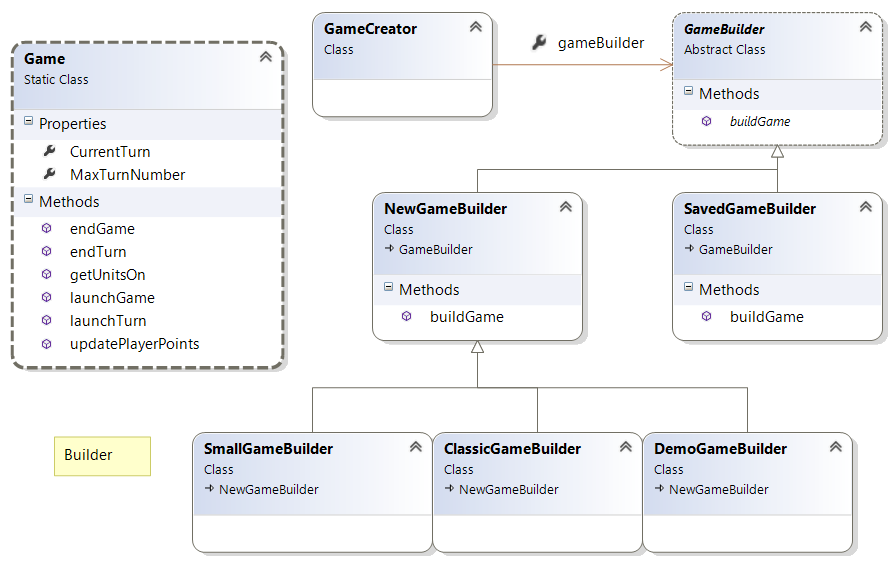
\includegraphics[width=1\textwidth]{figure/builder.png}
		\end{center}
		\caption{Création de la partie : patron de conception Monteur.}
		\label{fig:builder}
	\end{figure}


	\subsection{Fabrique : création des unités de chaque peuple}
		
		Chaque joueur possède une armée composée d'un certain nombre d'unités d'un même peuple. Ces unités sont soit des Elfes, soit des Humains, soit des Korrigans. Cette règle se traduit par un objet \emph{Player} qui possède une \emph{Faction}, elle même composé d'objets \emph{Units}. Cette modélisation est illustrée par la \textsc{Figure} \ref{fig:factory}. \emph{Units} est une classe abstraite implémentée par trois classes concrètes représentants les trois peuples disponibles. La création de ces unité est assurée par le patron de conception \textbf{Fabrique}. Ce patron de conception nous permettra de créer l'armée adéquate en fonction du peuple choisit par le joueur au lancement de la partie. Il assure une modularité du code, car sa fonction \emph{CreateUnit} retourne un type abstrait. Ainsi, l'appelant n'a pas besoin de se préoccuper de la classe concrète de l'objet retourné par cette méthode. 
		
		\begin{figure}[h]
			\begin{center}
				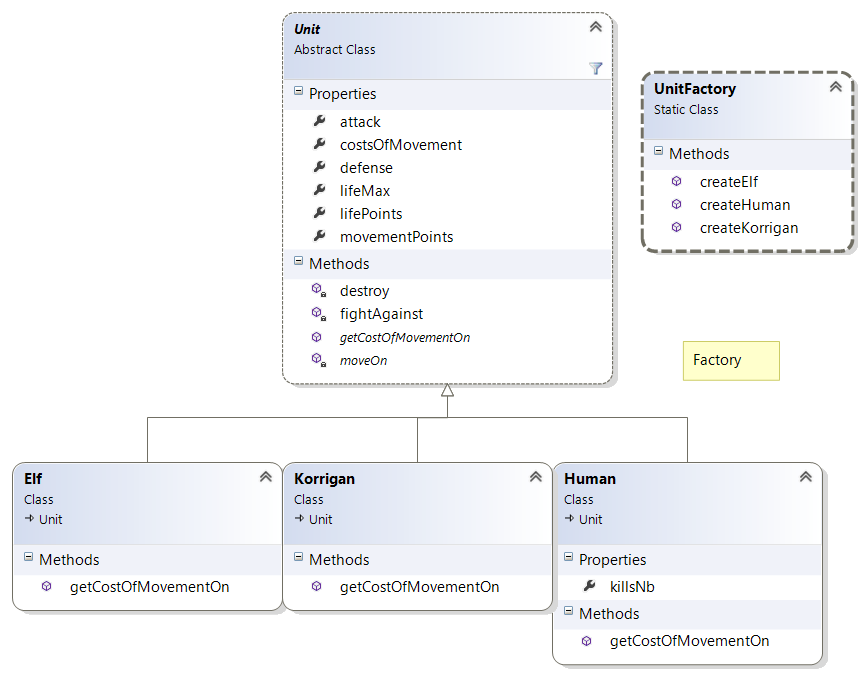
\includegraphics[width=1\textwidth]{figure/factory.png}
			\end{center}
			\caption{Création des unités : patron de conception Fabrique.}
			\label{fig:factory}
		\end{figure}


	\subsection{Poids-mouche : création des hexagones}

		La classe \emph{Game} possède un plateau \emph{Board}, composé de cases \emph{Hexagone}. Comme un plateau peut par exemple contenir 194 cases, l'ensemble des cases occuperait une grande quantité de mémoire si chaque case était instanciée une à une. Nous utilisons donc ici le patron de conception \textbf{Poids-mouche} représenté sur la \textsc{Figure} \ref{fig:flyweight} pour minimiser ces instances d'\emph{Hexagone}. La classe \emph{HexagonFactory} se charge de fournir les quatre types de cases lors de la création de la carte. Ainsi, pour chaque case du plateau, s'il s'agit d'un type de case qui n'a pas encore été instancié, il la fabrique ; sinon, il fournit simplement l'objet déjà existant. De cette manière, on représente un nombre importants de cases par la répétitions de seulement quatre instances : \emph{Woods, Mountains, Desert} et \emph{Plain}. Cette modélisation nous impose de ne pas implémenter de paramètres à l'objet \emph{Hexagone} car il serait similaire à toutes les cases de même type. Ainsi, ce seront les objets \emph{Units} qui connaitront leur position sur le plateau, et non pas les cases qui sauront quelles unités sont sur elles.

		\begin{figure}
			\begin{center}
				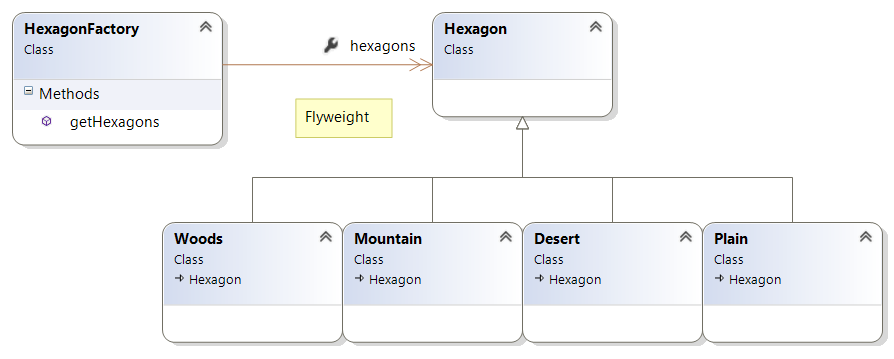
\includegraphics[width=1\textwidth]{figure/flyweight.png}
			\end{center}
			\caption{Gestion des cases : patron de conception Poids-mouche.}
			\label{fig:flyweight}
		\end{figure}


	\subsection{Stratégie : création des différents type de carte}

		Comme indiqué dans la Section \ref{subsec:carte}, il existe différentes tailles de cartes : Démo, Petite et Normale. La disposition des cases doit être décidée aléatoirement lors de la création d'une nouvelle carte, et ce indépendamment de sa taille.  De plus, le nombre de case doit être un multiple de 4, afin d'avoir autant de cases de type Desert, Forêt, Montagne et Plaine. Nous allons donc utiliser le patron de conception \textbf{Stratégie} pour l'initialisation d'une nouvelle carte. Comme le montre la \textsc{Figure} \ref{fig:strategy}, la classe \emph{Board} possède un attribut \emph{StrategyBoard} interchangeable qui définit la stratégie d'implémentation du plateau. 
		
		
		\begin{figure}
			\begin{center}
				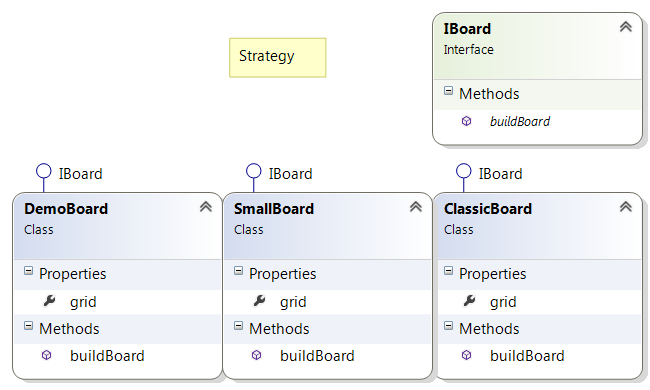
\includegraphics[width=0.7\textwidth]{figure/strategy.png}
			\end{center}
			\caption{Création des différents types de carte : patron de conception Stratégie.}
			\label{fig:strategy}
		\end{figure}






